\chapter{Funktionstest/Validierung}\label{chap:Funktionstest}
\thispagestyle{standard}
\pagestyle{standard}
\lfoot{\small Refik Kerimi}

\section{Ausgangsbedingung und Ausgrenzung}
Getestet werden die in Kapitel \ref{chab:Basistechnologien} beschriebenen Funktionen. Dies wurde zum einen über die DevTools vom Chrome Browser sowie über das Chrome PlugIN Lighthouse getestet. Weiters wurde die von der Emulator von Android Studio verwendet um den Test ohne Androidgerät darzustellen. Die Applikation selbst wurde hier nicht Behandelt.
Die 
 
\section{Testen auf Mobilen Gerät und Android Studio Emulator}
Um auf dem auf dem Mobilen \acl{SP} (\acs{SP}) Testen zu können muss der Developer Modus auf dem Gerät eingeschaltet werden. Dieses wird durch das aktivieren der Entwicklertools und USB-Debugging freigeschaltet wie in Abbildung \ref{fig:DevToolsAndorid} und \ref{fig:DevToolsChrome} zu sehen ist. 

\begin{figure}[h]
	\centering
	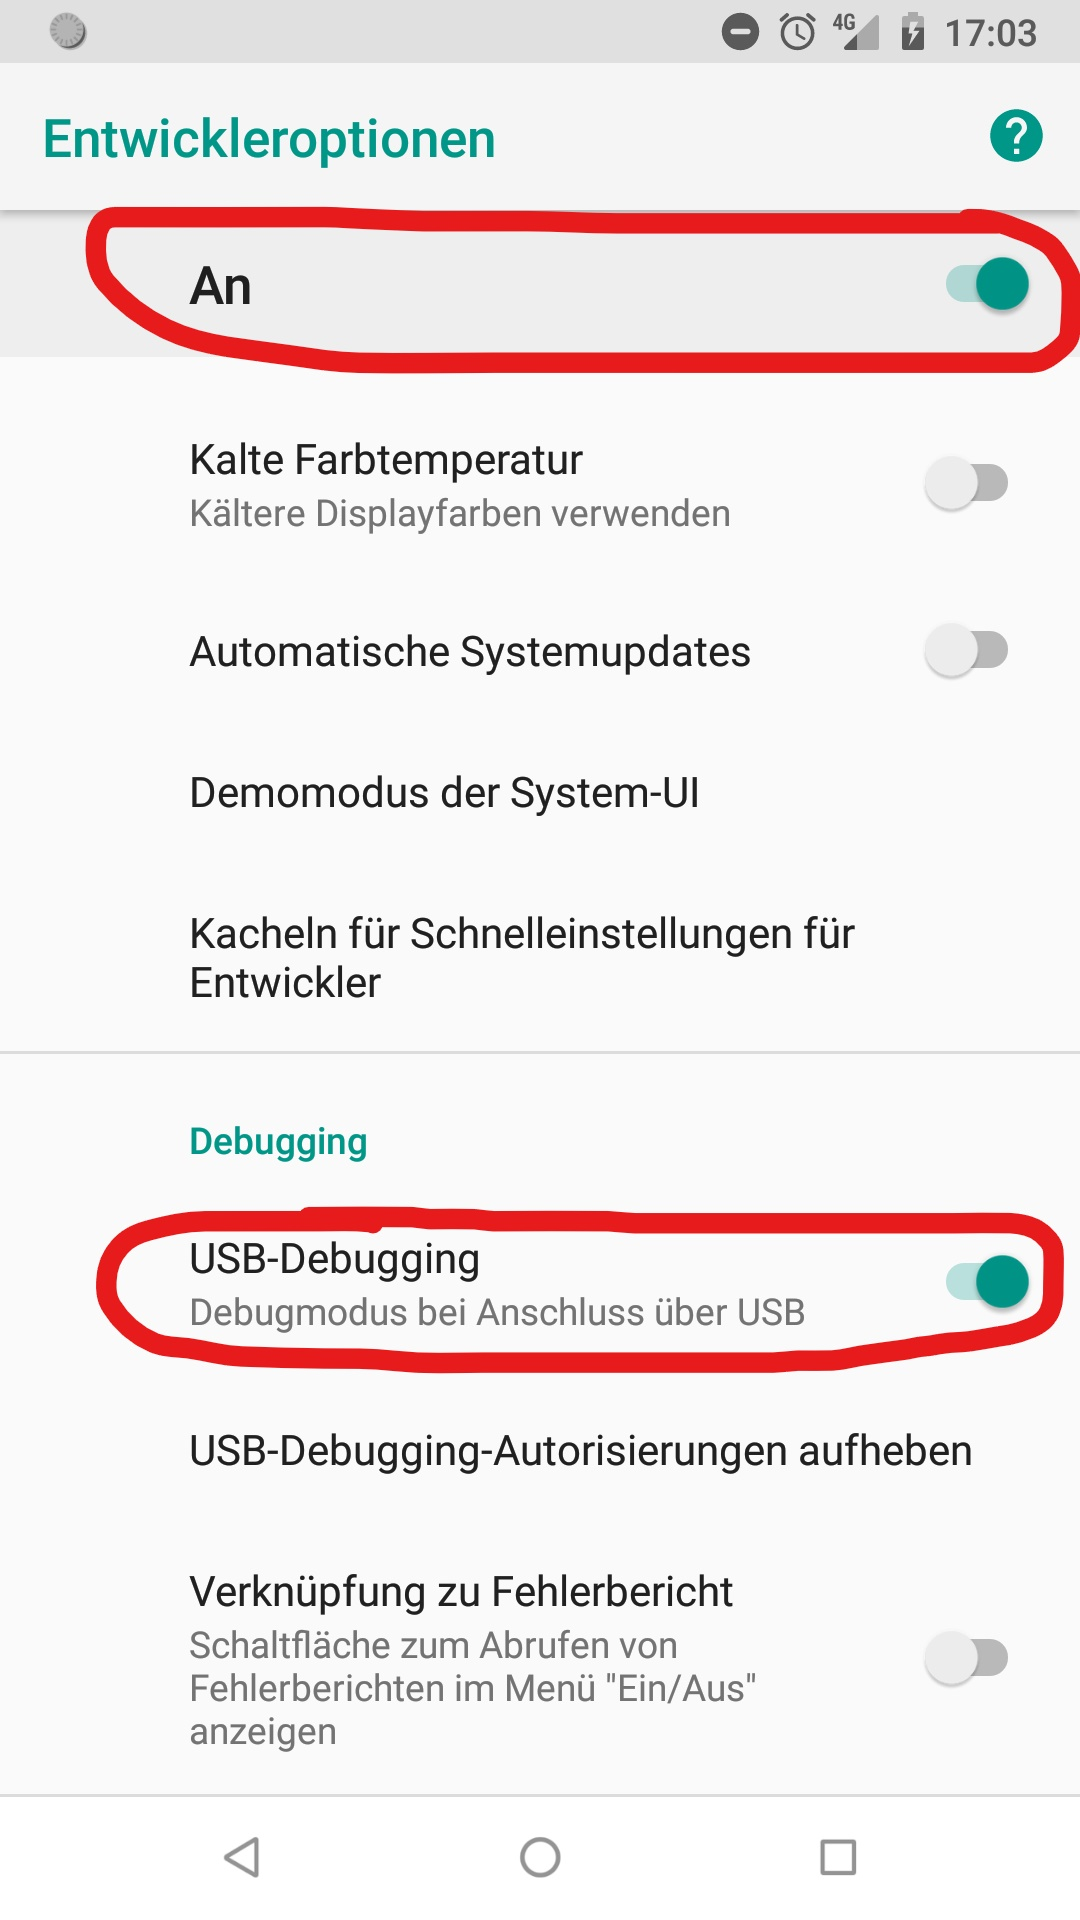
\includegraphics[width=6cm]{BilderAllgemein/DevToolsAndroid}\medskip
	\caption{Aktivieren der Entwicklertools auf Android 8.1.0}
	\label{fig:DevToolsAndorid}
\end{figure}

\begin{figure}[h]
	\centering
	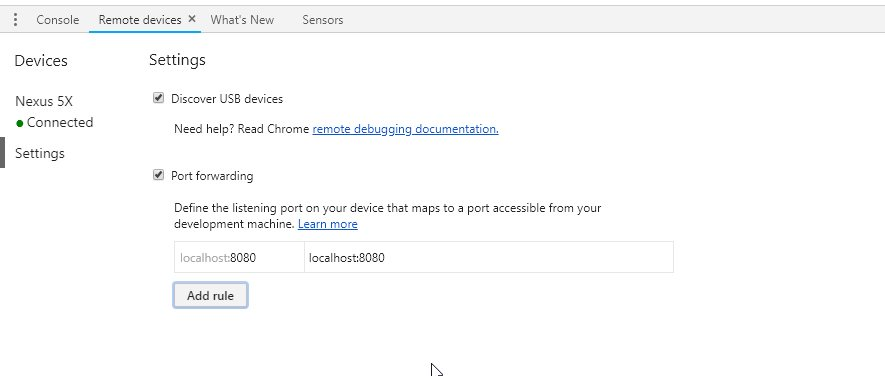
\includegraphics[width=14cm]{BilderAllgemein/DevToolsChrome}\medskip
	\caption{Anzeige der Verbindung auf Google Chrome 67}
	\label{fig:DevToolsChrome}
\end{figure}

Falls kein Android Gerät zur Verfügung steht ist der von Android Studio\footnote{https://developer.android.com/studio/} angebotene Emulator eine große Hilfe. Durch den integrierten Emulator lassen sich verschiedene Softwareversion von Android darstellen und helfen bei der Entwicklung und beim Testen der \acs{PWA}

\section{Lighthouse}
Lighthouse ist ein open-source Tool von Google und unterstützt den Entwickler bei der Verbesserung und Transformation der Applikation zu einer vollwärtigen \acs{PWA}. Man kann Lighthouse über 3 Wege verwenden:
\begin{itemize}
    \item  in Chrome DevTools
	\item  über die Kommandozeile
	\item  oder im Continues Integration Prozess als Node Module
\end{itemize}
Jeder dieser Workflows benötigt den Google Chrome Browser \cite{Lighthouse}.

\section{Komponententest}



\subsection{Add to Homescreen}



\subsection{Service Worker}



\subsection{Cache}



\subsection{Geolocation}




